\documentclass[10pt,a4paper,twocolumn]{article}
\usepackage[margin=18mm,columnsep=6mm]{geometry}
\usepackage[T1]{fontenc}
\usepackage{lmodern,amsmath,amssymb,graphicx,booktabs,microtype,url}
\usepackage[font=small,labelfont=bf]{caption}
\usepackage[colorlinks=true,urlcolor=blue,citecolor=blue]{hyperref}
\graphicspath{{figures/}{../10_METHOD_EVOLUTION_20261028/figures/}}
\hypersetup{pdftitle={When Do Legal Skill Parameters Improve Downstream Outcomes?},pdfauthor={ARES Research Working Group}}
\setlength{\parskip}{2pt}
\title{When Do Legal Skill Parameters Improve Downstream Outcomes?\\\large A Paired Physical Study of Residual Control, Parameterized PPO, and Outcome Selection}
\author{ARES Research Working Group\\\small Evidence-driven working manuscript, 28 October 2026}
\date{}
\begin{document}
\maketitle
\begin{abstract}
Residual control can rescue failures while regressing nominal successes. We investigate which legal skill parameters actually change subsequent physical outcomes, and whether observed execution effects help decide when to intervene. A bounded single-GPU study uses unmodified native ManiSkill tasks and actual SAPIEN/PhysX execution. Six ordinary PPO models consume 614,400 online control interactions. On the same 64 development conditions, ordinary residual PPO completes 63, 62, and 64 cases, versus 62, 63, and 60 for parameterized PPO. A train-only paired-outcome selector completes 60 cases, matching nominal control; fixed tuning and equal-collection-cost CEM complete 62. The parameter interface and conservative selection do not establish an independent algorithmic improvement. Peg insertion remains a weak baseline within its native budget. A physical pivot to StackPyramid demonstrates a first-skill parameter with both downstream rescue and regression, although its total success remains unchanged. We release reproducible scripts, measured trajectories, actual simulator videos, model hashes, and negative findings. These are state-based development experiments, not sealed-test, perception, or robot-transfer results.
\end{abstract}

\section{Question and contribution boundary}
The research question is whether legal parameter changes can improve the benefit--regression tradeoff of ordinary residual reinforcement learning. A nominal controller already solves many cases, so a small success increase can hide avoidable damage to successful executions. A useful mechanism must improve beyond strong fixed tuning, ordinary PPO, and a capacity-matched outcome predictor. It must also act through parameters that affect physical objects, rather than merely issuing a different desired trajectory.

Our contribution at this stage is an auditable physical study and an unsupported pilot hypothesis, not a new winning algorithm. We retire the earlier execution-active likelihood experiment: its actor gradients changed, but it did not yield stable gains. No new inactive-dimension PPO objective is trained here. The newly tested selector is a one-boundary contextual bandit, not a long-horizon semi-Markov policy. Sealed test cases remain unopened.

\section{Related mechanisms and competing explanations}
Parameterized primitives already appear in RAPS~\cite{raps}. STAP combines downstream skill values with parameter search and uncertainty~\cite{stap}. Fabrica uses task geometry and residual policies~\cite{fabrica}; Foresight Residual RL uses downstream success information~\cite{foresight}. SCOUT studies action--outcome feedback for adaptation~\cite{scout}. Action-space design itself can alter learnability~\cite{action}, and recovery chaining already learns to recover nominal skills~\cite{recovery}. We inspected available primary pages and selected public implementation paths; this does not constitute a reproduction of these algorithms. The supplied U-GRA publisher page could not be independently inspected because of HTTP 429, so no novelty distinction from its full method is claimed.

These precedents rule out calling a parameter interface, execution-history input, ensemble gate, or downstream predictor a novel method by itself. Our paired-difference hypothesis requires measurable benefit beyond a same-capacity absolute-outcome model on conditions excluded from model fitting. It fails that test in the present development study.

\section{Native tasks and legal authority}
We pin ManiSkill source commit \texttt{62ff3a58} and use SAPIEN 3.0.3, Torch 2.7.0+cu128, and one RTX 3080. Native physics, reward definitions, success predicates, and limits are unchanged. StackCube has 50 control steps at20Hz, PegInsertionSide100, and StackPyramid250. Pyramid's actual native horizon is250, not the Peg horizon. Evaluation uses native terminal success at the actual program end within the cap; Stack comparisons always execute all50 steps. A transient earlier success is not substituted for terminal success.

For Stack, the nominal Cartesian feedback program approaches, descends, closes, lifts, pre-places, lowers, opens, and retreats. Parameterized PPO outputs normalized $\xi\in[-1,1]^3$: placement $x/y$ offsets bounded by 15 mm and lower/release height bounded by 12 mm. Each offset enters the relevant skill target; the height offset is consumed only during lowering/release phases. Ordinary residual PPO instead modifies the native three-axis command and gripper command by a bounded 0.15 residual at every phase. Its authority is broader; this is an interface comparison, not an isolated new loss comparison. The parameter PPO comparator and the paired selector share the legal parameter controller.

All observations are explicitly state-based: robot joints, object and goal poses, current phase, previous measured object displacement, issued parameter history, and remaining budget. They contain privileged simulator state and are not a deployed perception interface. Request, clipping, actual parameter consumption, target, and measured object motion are logged. A post-training audit correction distinguishes issued height history from consumed height in inactive phases. It changes only logging, not actions or actor observations. Exact training sources are frozen alongside model hashes.

\begin{figure*}[t]
\centering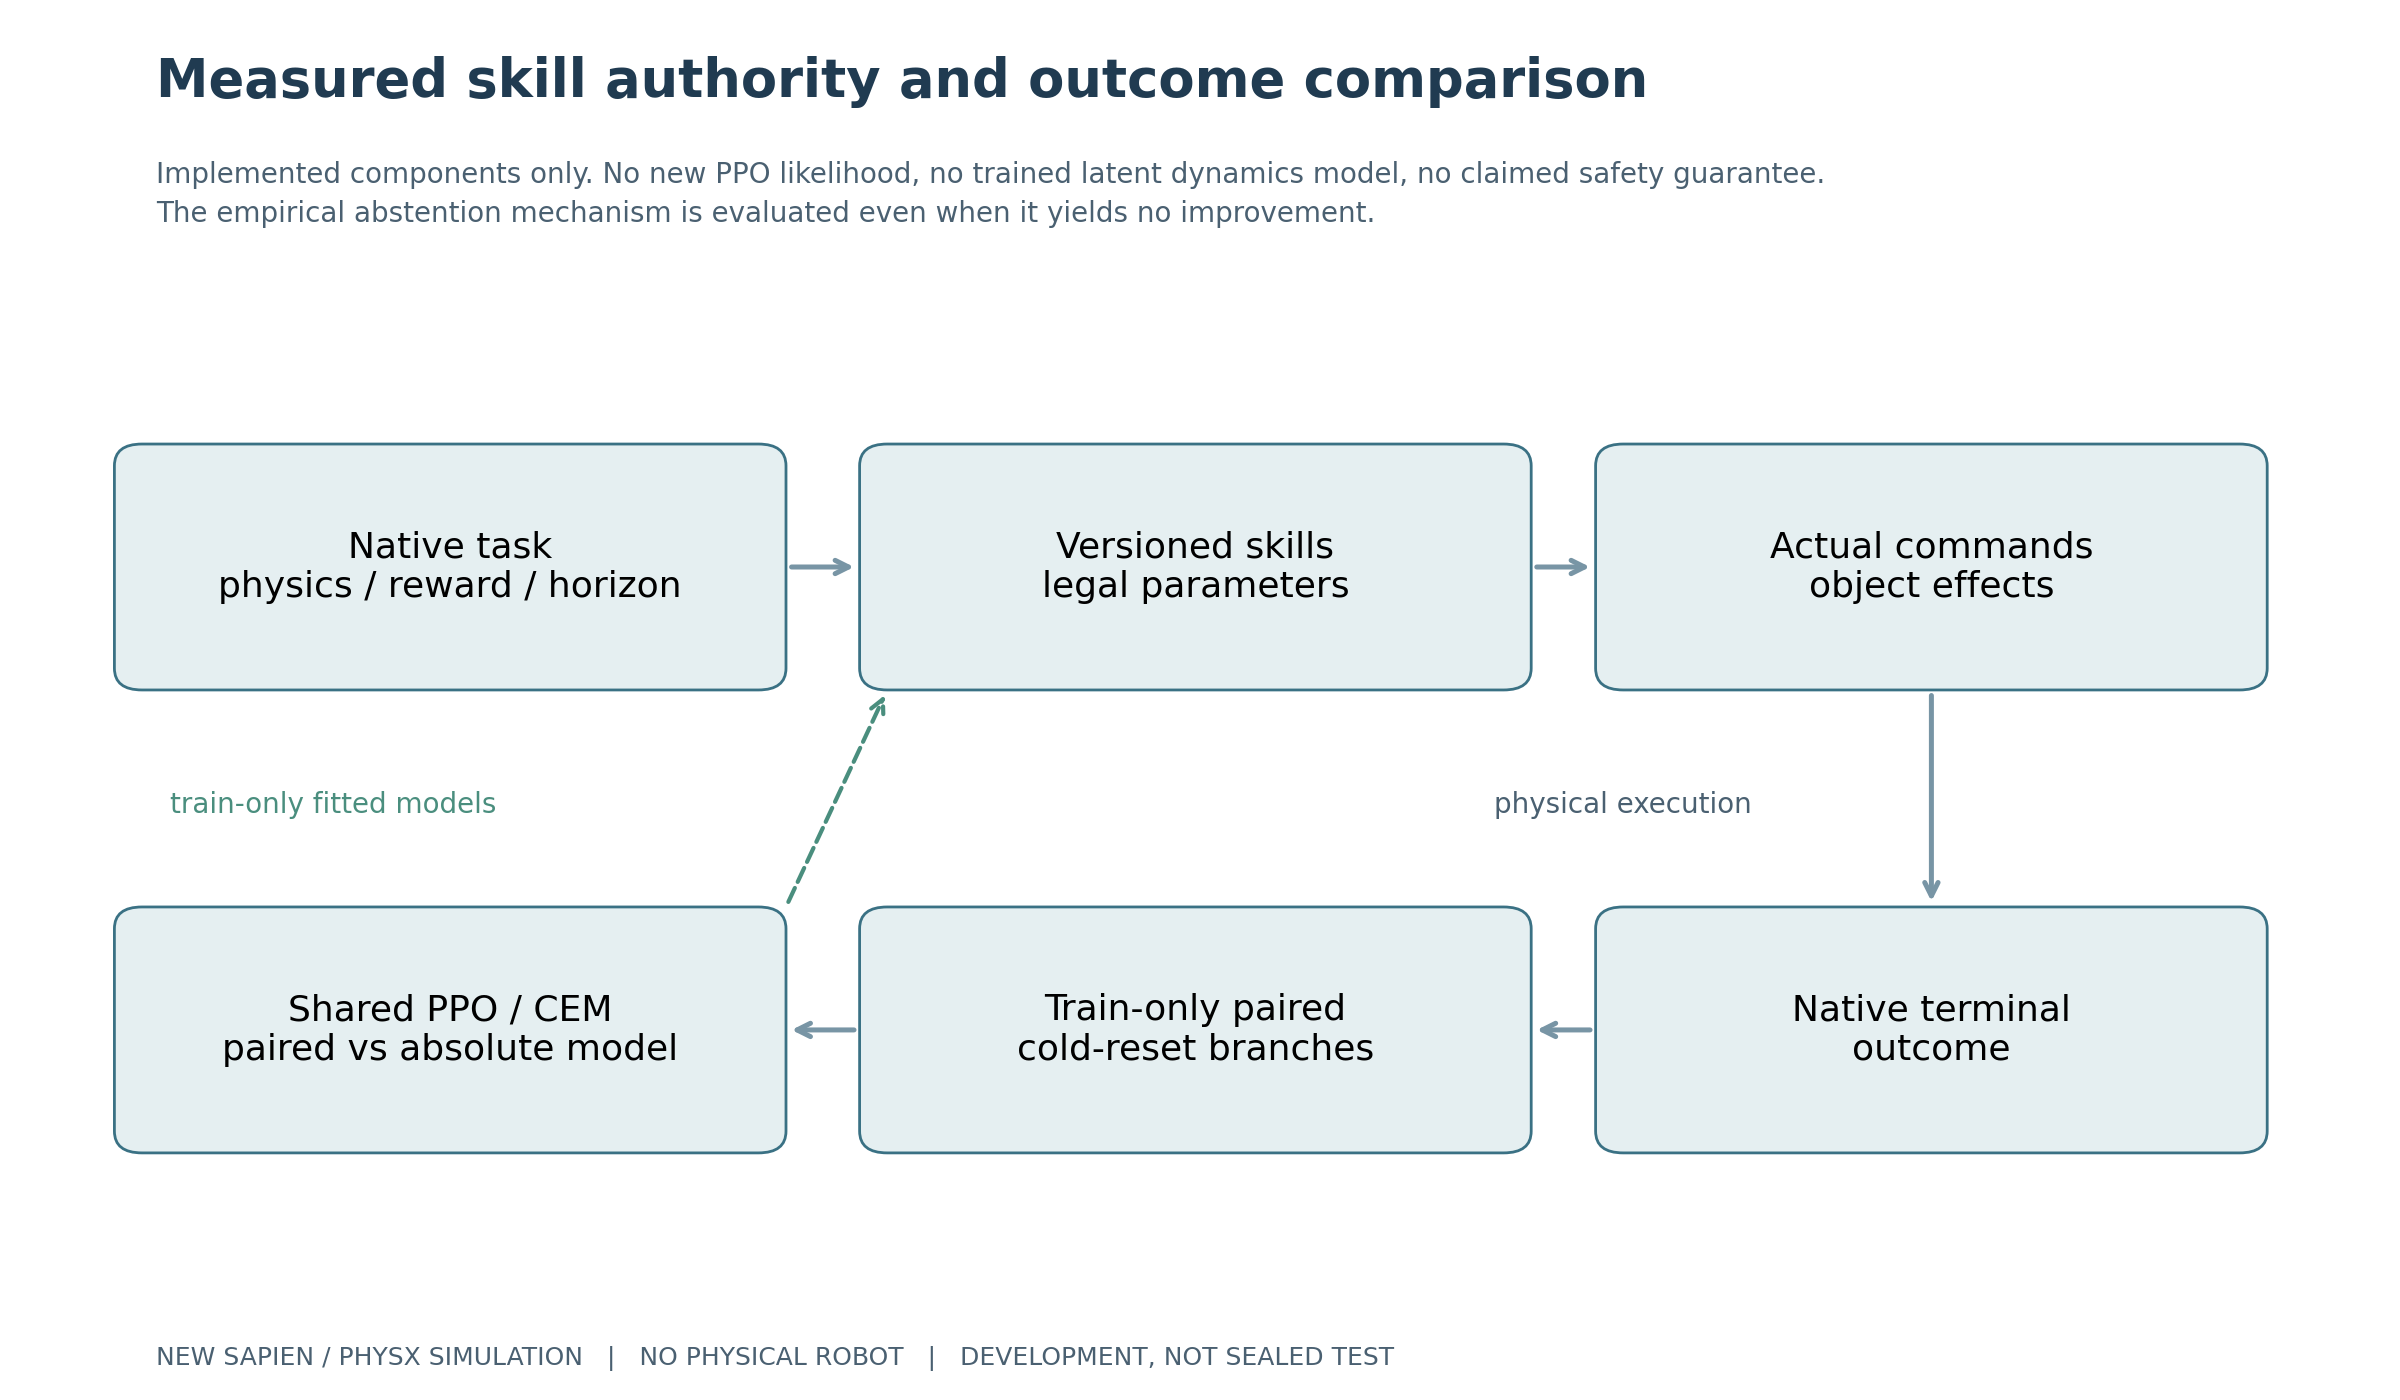
\includegraphics[width=.94\textwidth]{Fig1_system.png}
\caption{Implemented physical evidence pipeline. All branches are actual native simulator executions. Training-only cold resets obtain outcome labels; deployment decisions use only currently available state and past effects. There is no real-robot motion.}
\label{fig:system}
\end{figure*}

\section{Outcome comparison and conservative choice}
At the first legal place boundary, context $o$ includes robot/object relative state, preceding observed displacement, the next goal, and remaining control budget. On independent training conditions we cold-reset and execute nominal, lower 12 mm, and higher 12 mm branches. Initial hashes and the pre-decision physical prefix are checked. Each full suffix produces native outcome $Y_j$. The implemented target is
\begin{equation}
D_j(o)=Y_j-Y_0,\qquad j\in\{\mathrm{lower}, \mathrm{higher}\}.
\end{equation}
All Stack branches execute 50 steps, so actual execution-time differences are zero; $\lambda_T=0$. Earlier stable completion is retained as a diagnostic, not counted as saved execution time. No branch is restored to a shared successor state after the actions diverge.

Five bootstrap MLPs (two 64-unit hidden layers each) predict three outcomes: zero nominal advantage and two differences. A candidate is selected only when its empirical mean minus one ensemble standard deviation exceeds 0.05; otherwise the nominal skill is retained. This threshold is fixed before development evaluation. It is an empirical abstention rule, not a calibrated probability or a formal safety guarantee. The same-capacity absolute-outcome baseline predicts $Y_j$ and subtracts its predicted nominal value. Ablations remove previous effects, next-contract information, pairing, abstention, or ensemble uncertainty. Without a legal decision boundary, execution remains nominal.

\section{Protocol and cost accounting}
Training conditions are seeds 100000--100511; the development pool is 200000--200127 and sealed seeds 300000--300255 are never run. Split hashes were frozen before training. The reported 64 cases use the first half of the development pool. Upstream PPO monitoring samples the development pool, so these results are \emph{development}, not untouched test generalization. No development outcomes fit selector weights.

For each of three training seeds 31/37/43, both PPO interfaces receive 102,400 online interactions: 614,400 total. We use the pinned upstream ordinary PPO implementation with identical three 256-unit actor/critic networks, 50-step rollouts, 64 environments, eight minibatches, and the native dense reward. A failed initial launch due to partial-reset configuration performs zero control steps and is preserved separately. Final actors differ from their initial weights and are actually executed in new paired evaluations.

Paired supervision costs $512\times 3\times 50=76,800$ actual interactions. Of 512 conditions, 507 reach a legal decision boundary:380 fit conditions and 127 calibration conditions, partitioned within the training pool. Five do not yield a decision label. A global height CEM receives the same 76,800 collection cost (16 candidates, 96 training conditions each); it chooses one fixed parameter on training conditions, not a per-development-case oracle. This matches collection cost, not the total PPO learning budget. Every probe, evaluation, monitoring rollout, and video rerun is separately counted in the released cost ledger.

Cold-reset hash equality is enforced per policy and case group. Parallel reset groups contain 16 cases; groups and training seeds, rather than $3\times 64$ supposedly independent scenes, define the uncertainty calculation. A paired hierarchical bootstrap resamples three model seeds and four shared groups. With so few groups its interval is only descriptive, not strong inferential evidence. Some jobs share GPU 0; their wall times do not establish algorithmic speed differences.

\section{Measured results}
\subsection{Parameterized control does not beat residual PPO}
Table~\ref{tab:main} retains every seed and ablation. Parameter minus residual mean success is $-2.08$ percentage points, with a descriptive paired hierarchical 95\% interval of $[-6.25,+4.17]$. One parameter seed has no regressions, but another loses four successes relative to its residual counterpart. There is no stable new-interface advantage. Actual learning curves and actor-update norms accompany the checkpoints.

\begin{table*}[t]\centering\small
\IfFileExists{RESULTS_TABLE.tex}{\begin{tabular}{lrrrl}\toprule
Policy & Success & Rescue & Regress & $\Delta$pp [95\% grouped CI] \\
\midrule
nominal & 60/64 & 0 & 0 & +0.00 [+0.00, +0.00] \\
fixed\_height\_minus & 62/64 & 3 & 1 & +3.12 [-3.12, +9.38] \\
fixed\_height\_plus & 62/64 & 3 & 1 & +3.12 [+0.00, +6.25] \\
residual\_ppo\_31 & 63/64 & 4 & 1 & +4.69 [-3.12, +10.94] \\
parameter\_ppo\_31 & 62/64 & 3 & 1 & +3.12 [-3.12, +9.38] \\
residual\_ppo\_37 & 62/64 & 4 & 2 & +3.12 [-7.81, +10.94] \\
parameter\_ppo\_37 & 63/64 & 3 & 0 & +4.69 [+0.00, +9.38] \\
residual\_ppo\_43 & 64/64 & 4 & 0 & +6.25 [+1.56, +10.94] \\
parameter\_ppo\_43 & 60/64 & 2 & 2 & +0.00 [-4.69, +4.69] \\
paired & 60/64 & 0 & 0 & +0.00 [+0.00, +0.00] \\
no\_effect & 60/64 & 0 & 0 & +0.00 [+0.00, +0.00] \\
no\_next\_contract & 59/64 & 0 & 1 & -1.56 [-4.69, +0.00] \\
no\_pairing & 60/64 & 0 & 0 & +0.00 [+0.00, +0.00] \\
no\_abstain & 62/64 & 3 & 1 & +3.12 [+0.00, +6.25] \\
no\_uncertainty & 61/64 & 1 & 0 & +1.56 [+0.00, +4.69] \\
cem\_global\_height & 62/64 & 2 & 0 & +3.12 [+0.00, +6.25] \\
\bottomrule\end{tabular}
}{\begin{tabular}{lrrrl}\toprule
Policy & Success & Rescue & Regress & $\Delta$pp [95\% grouped CI] \\
\midrule
nominal & 60/64 & 0 & 0 & +0.00 [+0.00, +0.00] \\
fixed\_height\_minus & 62/64 & 3 & 1 & +3.12 [-3.12, +9.38] \\
fixed\_height\_plus & 62/64 & 3 & 1 & +3.12 [+0.00, +6.25] \\
residual\_ppo\_31 & 63/64 & 4 & 1 & +4.69 [-3.12, +10.94] \\
parameter\_ppo\_31 & 62/64 & 3 & 1 & +3.12 [-3.12, +9.38] \\
residual\_ppo\_37 & 62/64 & 4 & 2 & +3.12 [-7.81, +10.94] \\
parameter\_ppo\_37 & 63/64 & 3 & 0 & +4.69 [+0.00, +9.38] \\
residual\_ppo\_43 & 64/64 & 4 & 0 & +6.25 [+1.56, +10.94] \\
parameter\_ppo\_43 & 60/64 & 2 & 2 & +0.00 [-4.69, +4.69] \\
paired & 60/64 & 0 & 0 & +0.00 [+0.00, +0.00] \\
no\_effect & 60/64 & 0 & 0 & +0.00 [+0.00, +0.00] \\
no\_next\_contract & 59/64 & 0 & 1 & -1.56 [-4.69, +0.00] \\
no\_pairing & 60/64 & 0 & 0 & +0.00 [+0.00, +0.00] \\
no\_abstain & 62/64 & 3 & 1 & +3.12 [+0.00, +6.25] \\
no\_uncertainty & 61/64 & 1 & 0 & +1.56 [+0.00, +4.69] \\
cem\_global\_height & 62/64 & 2 & 0 & +3.12 [+0.00, +6.25] \\
\bottomrule\end{tabular}
}
\caption{Native Stack development outcomes on the same 64 conditions. Rescue and regression are relative to nominal. Intervals resample the four shared reset groups and are descriptive. Counts are paired; rows are not independent scene samples.}
\label{tab:main}\end{table*}

\subsection{Paired abstention has no independent benefit}
The paired selector matches nominal 60/64 and rescues no nominal failures. Removing abstention gives 62/64 but incurs one regression. Removing the next contract yields 59/64. The same-capacity absolute predictor matches 60/64. Its calibration difference MSE (0.02895) is lower than the paired model's 0.03701; the prediction label alone does not establish a better decision mechanism. Fixed tuning and CEM reach 62/64. These are competing explanations for small gains, not weak baselines to omit.

\begin{figure}[t]\centering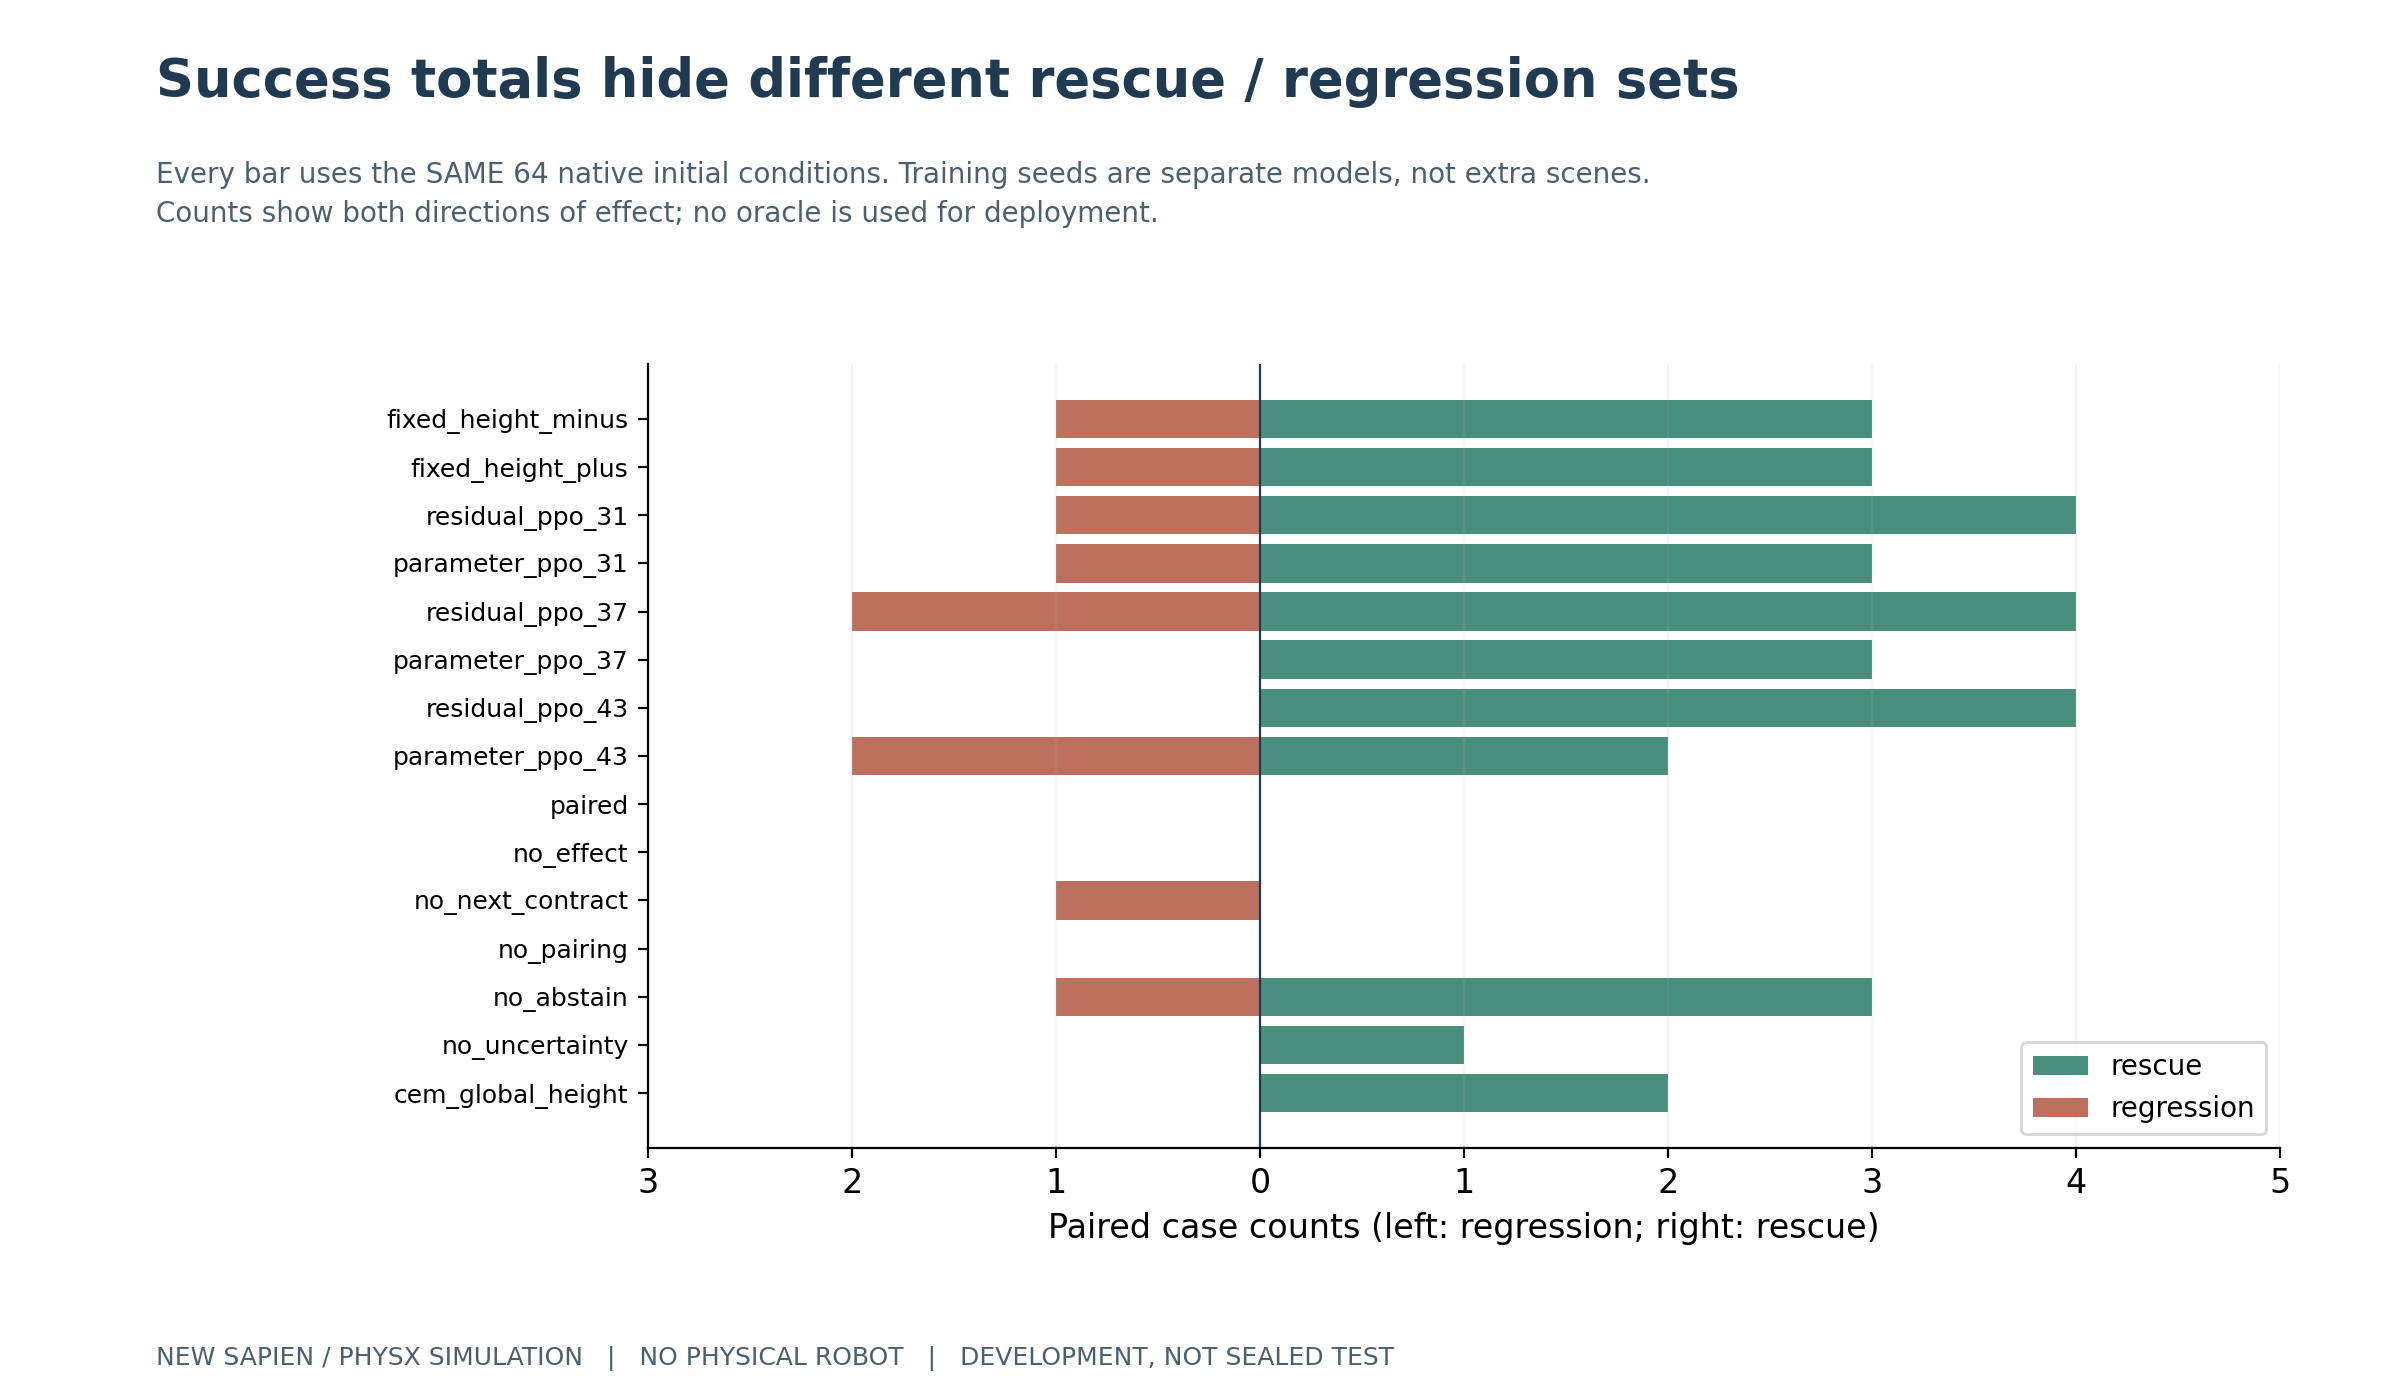
\includegraphics[width=\columnwidth]{Fig6b_paired_tradeoff.png}
\caption{Rescue and regression counts for all policies. A success total alone conceals interventions that help one case and damage another.}
\end{figure}

\subsection{Peg requires a credible physical baseline}
Eight design conditions test the official planner, faster legal timing/refinement, and observed final correction. Initial variants all yield 0/8 within the native 100-step cap. Path stride and bounded joint-readback tracking yield 1/8. A subsequent reactive insertion and align-before-advance round also yield 1/8. Actual joint velocity, peg/hole error, grasp, and phase traces expose tracking/contact failures. No episode is extended to claim official success, and a zero baseline is not used to advertise RL improvement. Peg RL is deferred until grasp/orientation/entry tracking becomes reliable. These eight cases are a design pilot, not a benchmark claim.

\subsection{A multi-stage physical pivot, not another RL win}
A handwritten Pyramid controller yields 0/16 and is rejected as a weak comparator. With the pinned official planner and a current-GPU pose adapter, four new single-environment conditions complete 4/4, both with ordinary path following and with stride-two bounded tracking. These are different conditions and reset arity from the failed handwritten probe, so the percentages are not a paired algorithm comparison.

A new 16-condition, single-environment paired probe then changes only the first cube-placement target $x$ by $\pm 12$mm. The later top-cube placement uses the actually observed base-cube poses. Nominal succeeds 12/16; minus 12 mm also 12/16 but has one rescue (case 122007) and one regression (122005); plus 12 mm succeeds 7/16 with five regressions. Identical initial hashes and actual state traces show a bidirectional first-skill effect on the downstream full task. This establishes a physical research opportunity, not a learned solution. Pyramid remains a stacking-family task; it does not satisfy a two-distinct-mechanism generalization claim.

A subsequent source audit found that the official program delays opening the first cube until the approach to the next grasp. We froze and ran a same-16-case control ablation that adds a native gripper-open immediately after the first goal. It yields 11/16 (one rescue, two regressions relative to nominal); the minus/plus offset variants each yield 9/16. Thus the simple release explanation also fails to improve total completion. Measured base-cube distances at first opening and task end are retained. Every native success in these paired probes also has the top cube more than 20 mm above both base cubes; this is an additional observed diagnostic, not a replacement native predicate. Including this ablation, all new training, probes, monitoring, evaluations, and video reruns consume 903,584 control interactions. No further learning is expanded on these design cases.

\begin{figure*}[t]\centering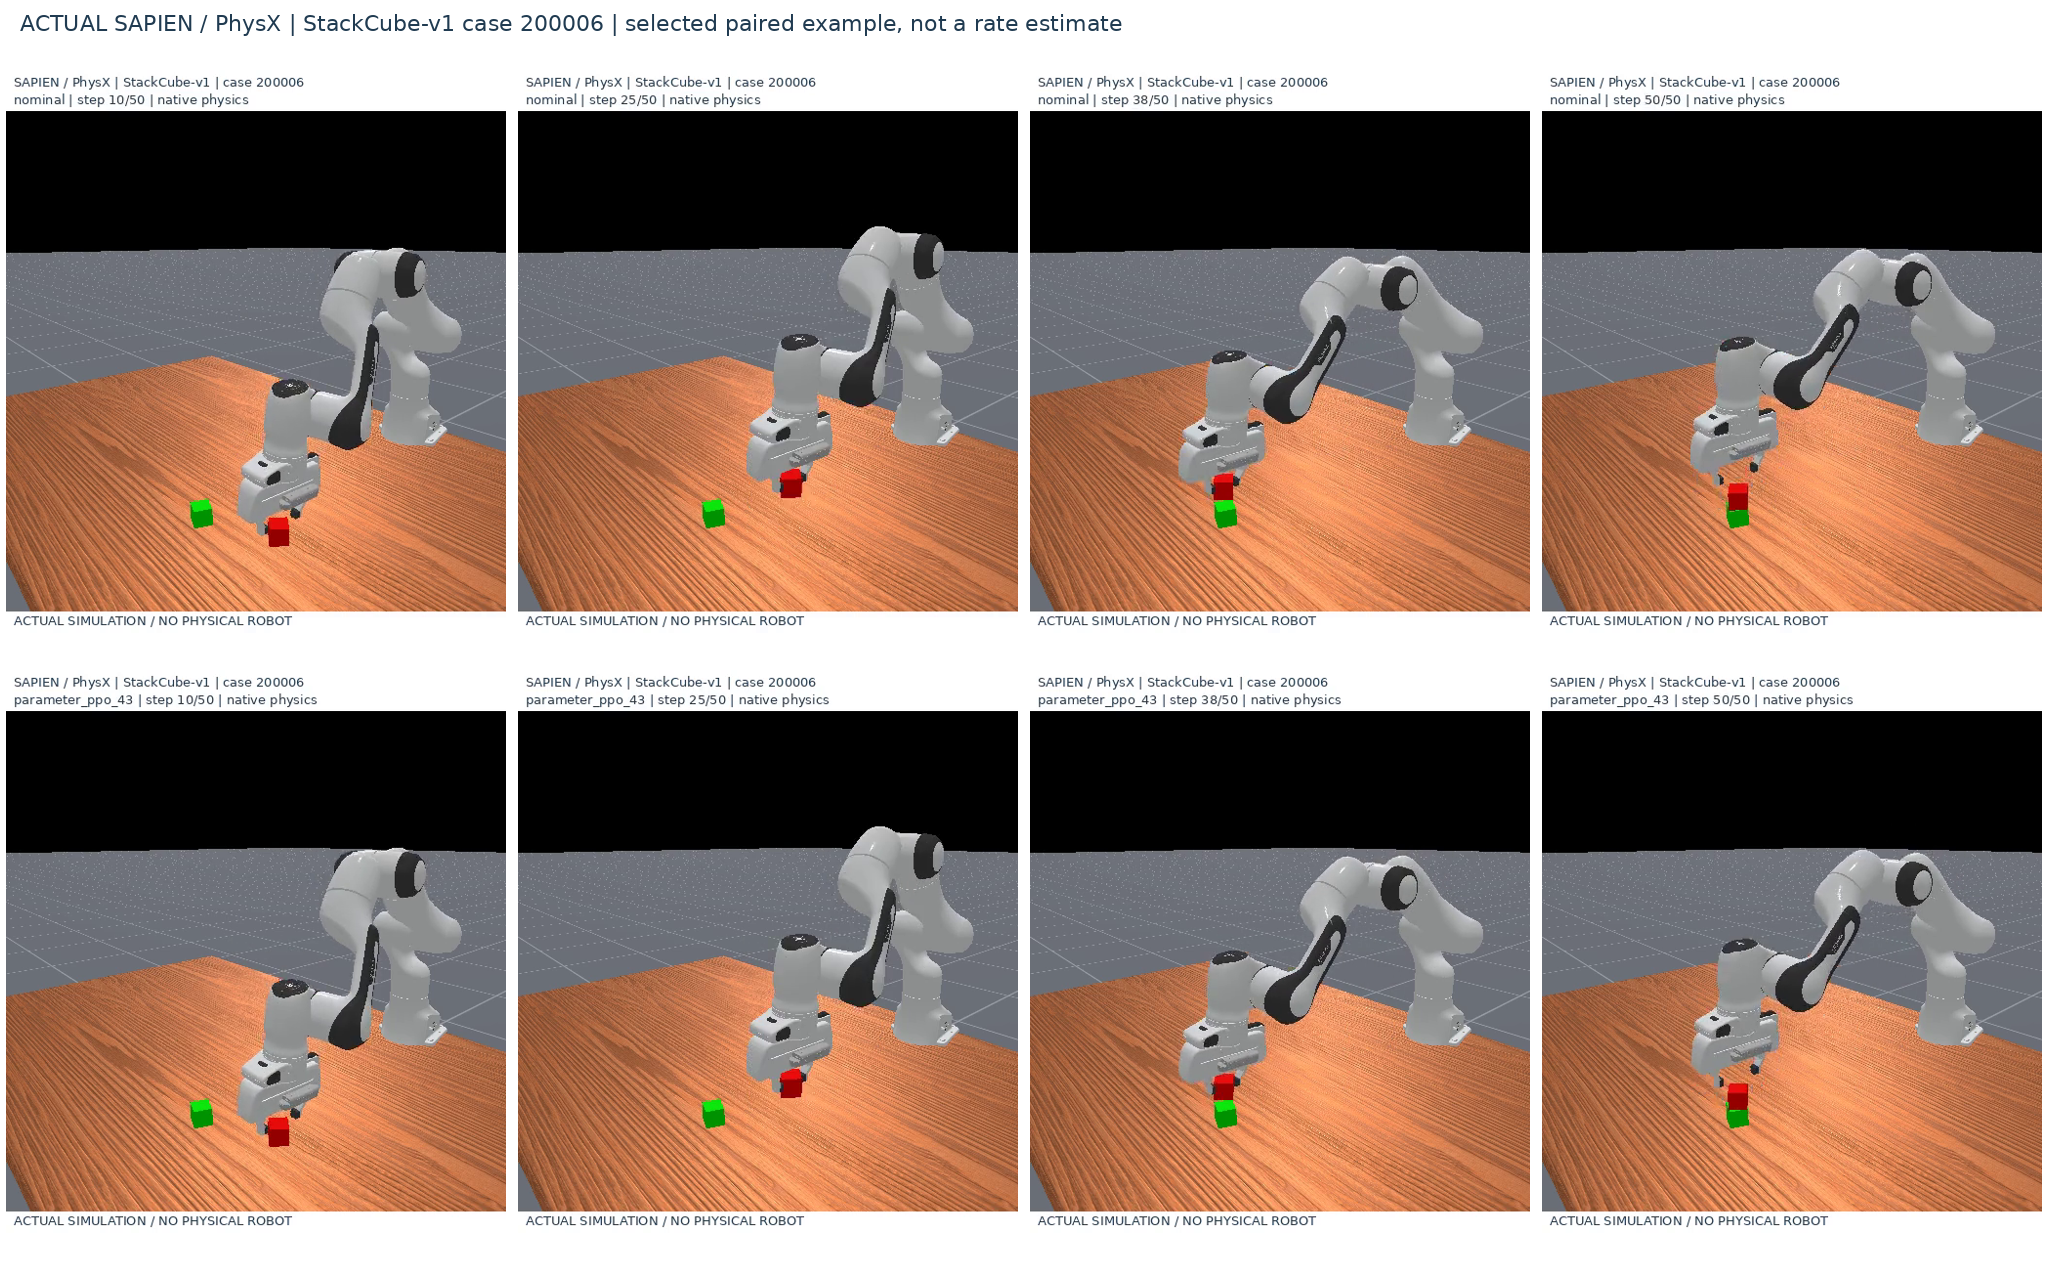
\includegraphics[width=.94\textwidth]{Fig3b_stack_regression.png}
\caption{Actual SAPIEN frames from the same Stack initial state (case 200006): nominal above, parameter PPO seed 43 below. This selected regression example is accompanied by a rescue example and complete case counts; it is not a rate estimate. Video reruns match primary initial hashes and outcomes.}
\end{figure*}

\section{Limitations and next falsifiable experiment}
This pilot does not deliver a mature SCI positive method. It uses only three model seeds, four development groups, privileged state, one shared GPU, and a small Pyramid design probe. Residual and parameter PPO have different control authority. Parameter PPO can update continuous XYZ every step; the selector makes one height-only choice. Thus PPO versus selector is not a matched action-frequency ablation. Only the paired and absolute predictors share the exact candidate set, boundary frequency, and capacity. A matched boundary-RL comparator remains unrun. The once-per-boundary selector is not long-horizon RL. There is no formal risk bound, deployed multimodal perception, JAKA success, or robot transfer. ARES-R stays read-only and no restricted site material enters this study. Public Panda assets cannot stand in for industrial geometry validation.

The next bounded experiment should freeze a Pyramid first-skill contract and compare same-authority ordinary parameter PPO, fixed/search control, absolute value, and paired difference choice on \emph{new} conditions. It should first verify that execution effects add predictive decision value beyond current geometry. Only a stable independent increment should trigger five-seed expansion and opening a newly sealed test. Peg should resume only after an independently credible native strong baseline. Without these results, the honest conclusion remains that legal control authority exists but the proposed learning mechanism is not established.

\section{Reproducibility and evidence}
The release contains protocol/split hashes, all policy/case paired outcomes, cost ledgers, measured learning curves, source freezes, actual simulator videos, individual PNG/SVG figures, and model/source indexes. Raw full trajectories and final models remain in a non-Git research bundle with SHA 256 and verified loaders. Paired clips preserve 20 Hz timing; a shorter completed program's final frame is held only for display and labeled accordingly. No state animation is represented as physical training. The companion HTML opens all evidence locally without a server.

\begin{thebibliography}{9}\small
\bibitem{raps} M. Dalal, D. Pathak, and R. Salakhutdinov. Accelerating Robotic Reinforcement Learning via Parameterized Action Primitives. NeurIPS34,2021. \url{https://proceedings.neurips.cc/paper_files/paper/2021/hash/b6846b0186a035fcc76b1b1d26fd42fa-Abstract.html}.
\bibitem{stap} STAP: Sequencing Task-Agnostic Policies. ICRA,2023. \url{https://sites.google.com/stanford.edu/stap/home}.
\bibitem{fabrica} Fabrica. CoRL,2025. \url{https://proceedings.mlr.press/v305/tian25a.html}.
\bibitem{foresight} Foresight Residual RL. arXiv:2607.16506,2026. \url{https://arxiv.org/abs/2607.16506}.
\bibitem{scout} SCOUT. arXiv:2609.36107,2026. \url{https://arxiv.org/abs/2609.36107}.
\bibitem{action} Demystifying Action Space Design. ICML,2026. \url{https://proceedings.mlr.press/v306/feng26ab.html}.
\bibitem{recovery} Recovery Chaining, public implementation. \url{https://github.com/shivamvats/recovery-chaining}.
\end{thebibliography}
\end{document}
